
\section*{Background}

The conclusions and implications of this think piece are built upon five key technical areas: Verification \& Validation, which is common in computer software and autonomy; correct by construction controllers which are generated with guarantees; probabilistic modeling of human decision making; collaborative autonomy, and model based system engineering. Each of these are briefly described here, with a few example references. 

\subsection*{Verification \& Validation (software v. autonomy)}

A recent study by the Office of the US Air Force Chief Scientist~\cite{tech-horizons2011} cited Verification and Validation (V\&V) is a key limitation in the ability to achieve the high impact gains that can be realized from autonomy. 
\begin{center}
\parbox[c]{6in}{
{\em ``Increased use of autonomy$\ldots$  will depend on development of entirely new methods for enabling `trust in autonomy' through verification and validation (V\&V) of the near-infinite state systems that result from high levels of adaptability and autonomy.''} \\
\hspace*{20pt} A Vision for Air Force Science and Technology 2010-30, USAF Chief Scientist, 2011.
}
\end{center}

It is important to first understand the definitions of Verification and Validation:
\begin{center}
\parbox[c]{6in}{
{\em Verification: Requirements evaluation {\em during} development} \\[0.1 in]
{\em Validation: Requirements evaluation {\em after} integration} %\\
%\hspace*{20pt} A Vision for Air Force Science and Technology 2010-30, USAF Chief Scientist, 2011.
}
\end{center}
Thus, the process of verification is to incrementally and systematically evaluate whether a system or subsystem is meeting requirements during the design process. Validation, on the other hand, evaluates whether the completed system meets the end customer requirements in a practical setting. If done well, Verification can speed up of the Validation process because portions of the underlying system have already been verified. 

The process of V\&V has been known for a long time, and is a formal part of nearly any systems engineering process~\cite{syseng-book}. The importance  of systematic processes has increased as the complexity/safety/security of the system has increased, such as in cars, airplanes, and spacecraft. V\&V for these systems has typically taken the form of empirical testing because it is closer to the end operational state, and people typically accept empirical testing easier than other options such as simulations. 

Most of these complex systems have grown in complexity more because of software growth than other components. Autonomous systems are particular challenging, as the physical system has not changed as much as the internal `intelligence' of the software. With the software growth, however, comes the typical challenges in verification of the system (now, a physical+software system). Dr.\ Werner Dahm, former Chief Scientist of the Air Force, has given several talks~\cite{gnc-talk} on the Air Force study in Ref.~citen{}, and cited the growth and errors in software. A small summary is given below:

\begin{table}
\begin{center}
\begin{tabular}{l|c}
System &  Lines of Code (loc)\\ \hline
F-4A & 1,000\\
F-15A &  50,000\\
F-16C &  300,000\\
F-22 &  2,500,000\\
F-35 &  18,000,000
\end{tabular}
\caption{Critical lines of code for aircraft; $\sim$4-6 errors per 1000 LOC, $\sim$0.1-1.0 errors per 1000 critical LOC}
   \label{table:loc}
\end{center}
\end{table}

Current V\&V methods are not sustainable as systems increase in complexity, given this growth. Dr.\ Dahm argues is that current systems with autonomous elements are tested to exhaustion of the budget, rather than to a formal level of V\&V. 

V\&V in software has also increased in importance over the years with the growth of programs and applications. Software companies... ({\bf Randal should write this, maybe mention beta testing, etc.}). 

With all applications, the time required for the processes for V\&V increases increases, creating pressures on safety/security/costs, etc. As such, recent research in the software engineering community has focused on developing automated, and formal, verification tools. (From the talk... Randal write...
- Model checking (Alloy, TLA+, VCC)
- Successful extensions to Internet scale (BGP, PAXOS))

The robotics community has borrowed/expanded these concepts for the verification of autonomy. In particular, research has been conducted in developing approaches for formal verification of software for autonomous systems. Spin~\cite{spin} and NuSVM~\cite{nusvm} are two examples of model checkers, which are designed to verify software which is typically generated from higher level specifications. The tools typically check logical consistency of a specification and reports on deadlocks, race conditions, incompleteness, and  assumptions. 

Most recently, the community has developed `probabilistic model checkers' which are designed to verify software to a particular level of probability. These tools typically verify a system through symbolic data structures and algorithms as well as exhaustive search. Importantly, atate of the art tools are being used to verify software and autonomy, even probabilistically.

\subsection*{Correct by construction controllers}

- summary here of Hadas’ stuff, others
- flow chart and example


\begin{figure}[h] 
\centering
   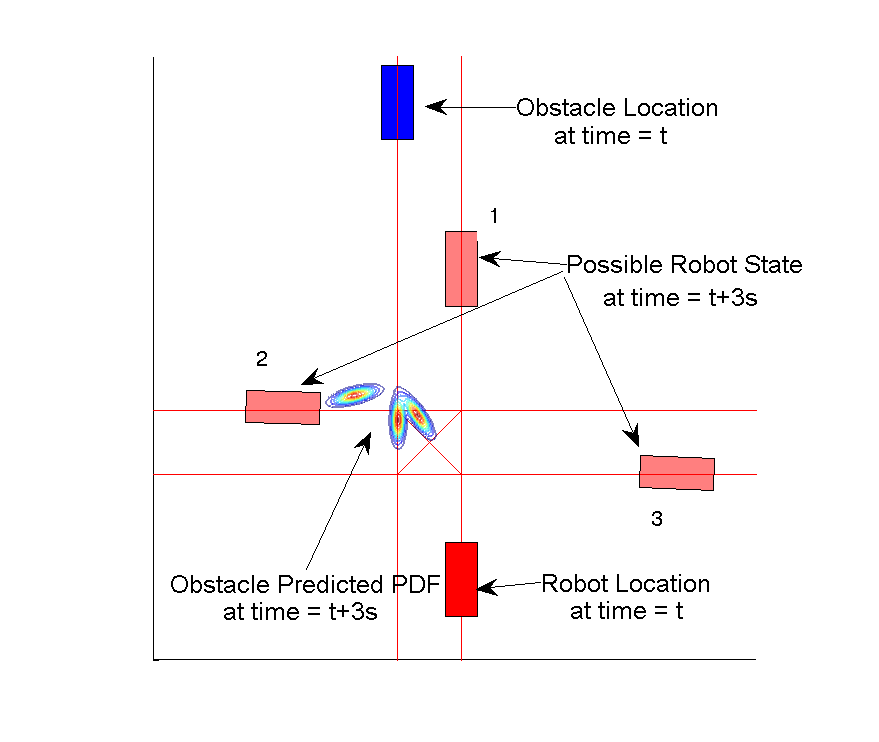
\includegraphics[width=3.0in]{coll_prob_inst.pdf} 
  % \label{fig:collision}
   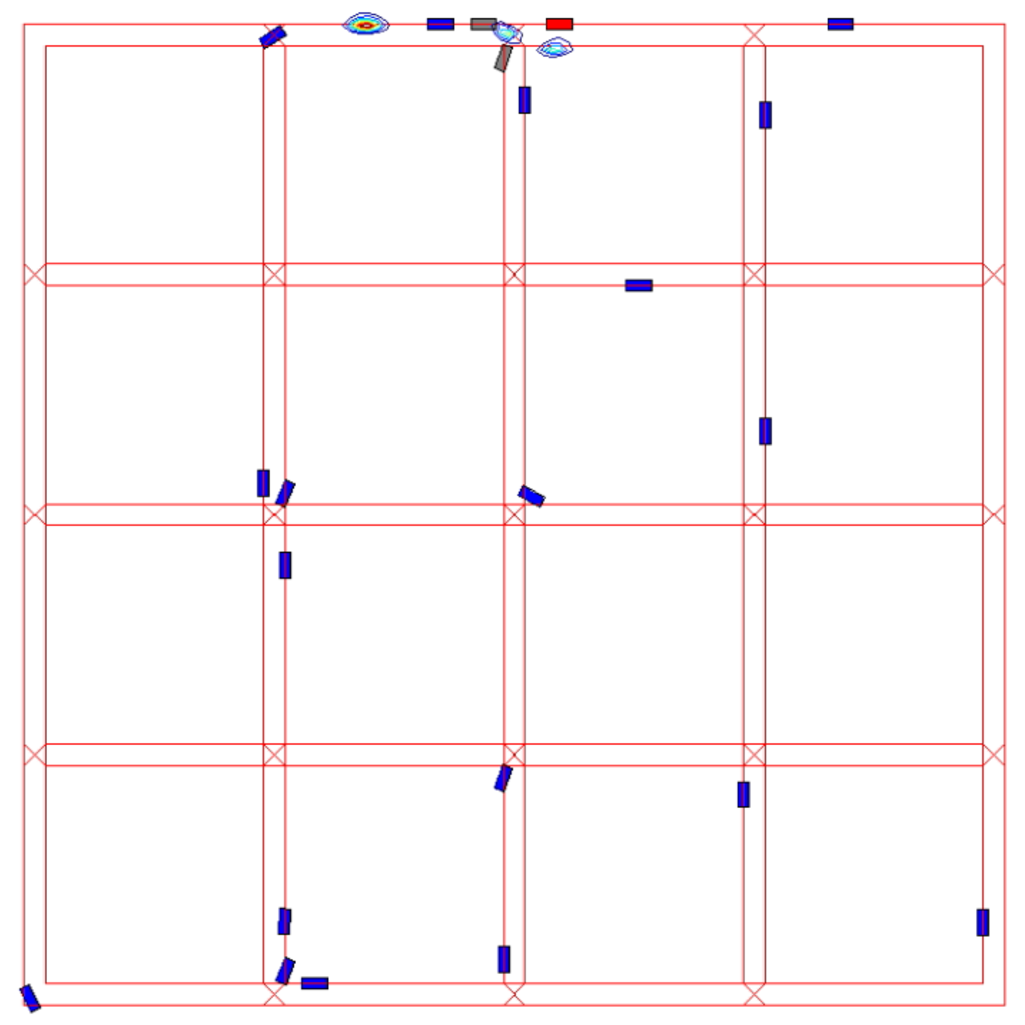
\includegraphics[width=2.5in]{taxi-driver.pdf} 
   \caption{collision probability taxi driver example}
   \label{fig:taxi-taxi}
\end{figure}




Can automatically develop  controllers (from models, high level specifications) that are probabilistically correct

\begin{figure}[h] 
\centering
   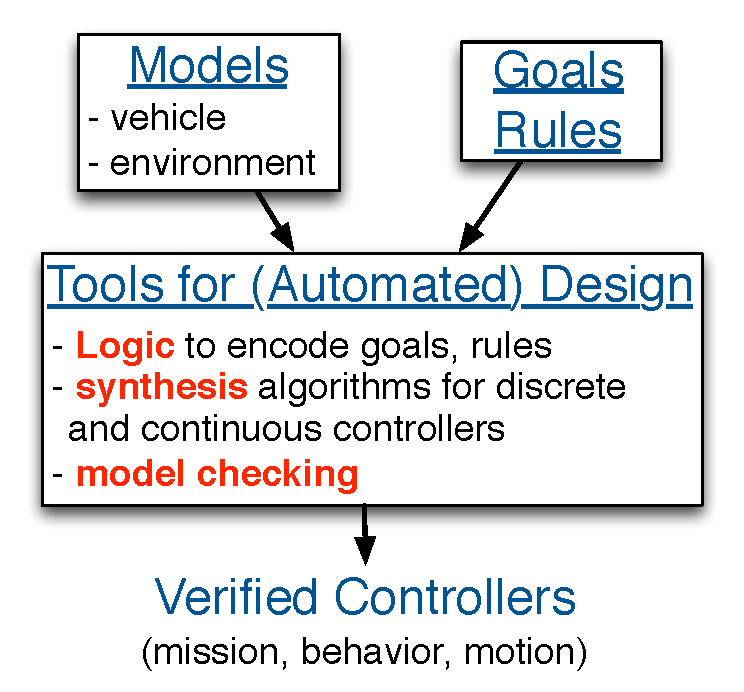
\includegraphics[width=2.5in]{correct-by-construction.pdf} 
   \caption{correct by construction example}
   \label{fig:correct-by-construction}
\end{figure}


\subsection*{Probabilistic modeling and humans}

Many types of models
Motor skills
     .
     .
     .
Bayesian Networks
Gaussian Processes
     .
     .
     .
ACT-R

Increasing in capabiolities complexity

Give GP example from Ergonomics


\begin{figure}[h] 
   \centering
   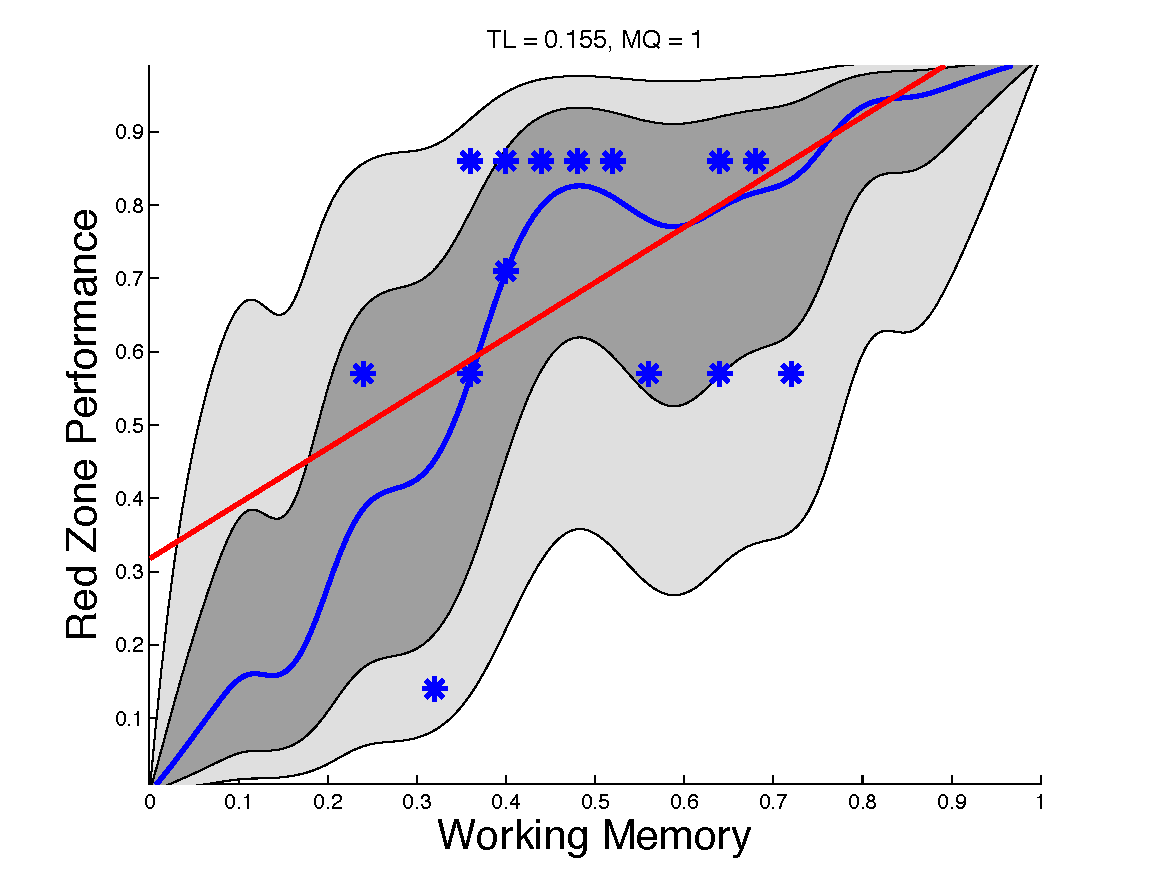
\includegraphics[width=3.5in]{GP-fig.pdf} 
   \caption{probabilistic modeling of human decision making example}
   \label{fig:prob-humans}
\end{figure}

There is a growing maturity in probabilistic models of human decision making


\subsection*{Collaborative autonomy}

Collaboration over computation, communication, navigation, and sensing

Multi-vehicle collaboration 
Decentralized task selection / allocation (Market protocols - Wellman et al, Optimization - How et al) 
Cooperative path planning (Tsourdos et al)
Scalability through swarm-based techniques (e.g., consensus, potential field)  (McLain et al)

Collaborative human-autonomy systems
Human intent prediction (e.g. partially-observable Markov Decision Process) (Karami et al)
Adaptive tasking (Parasuram et al)
Use metrics (e.g., confidence) to decide when to ask for help (Fong et al) 
Apply perspective-taking to project companion awareness state (Trafton et al)


Capable strategies for collaborative autonomy systems exist and can be 
leveraged for co-design of human-autonomy systems


\subsection*{Model-based system engineering}
Transition from functional decomposition..
Does not scale well
Difficult to verify


…to Model-based System Engineering 
State-based models of each actor are generated.
Each model is re-used over all phases of system engineering
Improves scalability and consistency
State analysis offers a formal method to verify behaviors
Successfully applied to single-actor systems (e.g., spacecraft missions)

